\section{Theorie}
\label{sec:Theorie}

% In knapper Form sind die physikalischen Grundlagen des Versuches, des Messverfahrens, sowie sämtliche für die Auswertung erforderlichen Gleichungen darzustellen. (Keine Herleitung)

% (eventuell die Aufgaben)

% Der Versuchsaufbau: Beschreibung des Versuchs und der Funktionsweise (mit Skizze/Bild/Foto)

\subsection{Aufbau einer Kathodenstrahlröhre}
\label{ssec:t1}

Die Ablenkung eines Elektronenstrahls in einem elektrischen Feld wird mit einer Kathodenstrahlröhre untersucht.
Diese besteht grundlegend aus drei verschiedenen Bauelementen.
Zu Beginn ist die "Elektronenkanone", oder auch braunsche Röhre. Sie emittiert freie Elektronen durch Glühemission durch die Öffnung eines Wehnelt-Zylinders hindurch.
Dieser besitzt eine elektromagnetishe Barriere, die von den Elektronen überwunden werden muss, da die Barriere durch eine Spannung $U_\text{C}$ kontrolliert werden kann, ist auch der Elektronenstrahl regelbar.
Nach dem Austritt werden die Elektronen auf eine Geschwindigkeit 

\begin{equation}
    v_\text{z} = \sqrt{\frac{2 \cdot e_0 \cdot U_\text{B}}{m_0}}
    \label{eq:zges}
\end{equation}

beschleunigt.
Dabei ist $e_0$ die Elementarladung und $m_0$ die Elektronenmasse. 
$U_\text{B}$ ist eine einstellebare Beschleunigungsspannung.
Die Elektronen passieren nach ihrem Austritt das Ablenksystem, zwei Plattenpaare, die jeweils senkrecht zueinander stehen.
Auf beide Paare wird eine elektrische Spannng angelegt, die passierende Elektronen ablenkt.
Schließlich landet der Strahl auf dem Leuchtschirm.
Dort regt der Strahl eine Reaktion an, die Lichtquanten freisetzt.
Der schematische Aufbau der Kathodenstrahlröhre ist in \autoref{fig:roehre} dargestellt.

\begin{figure}
    \centering
    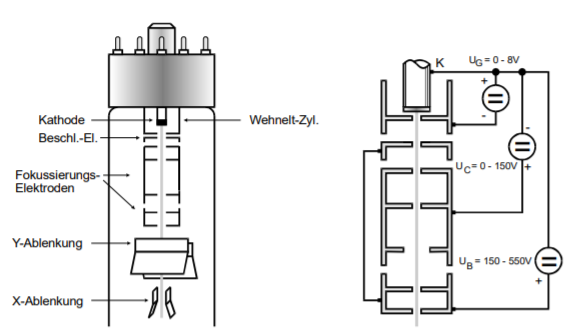
\includegraphics[width=\textwidth]{images/bild1.png}
    \caption{Schematischer Aufbau der Kathodenstrahlröhre.}
    \label{fig:roehre}
\end{figure}

\subsection{Berechnung der Ablenkung eines Elektronenstrahls im elektrischen Feld}
\label{ssec:t2}

In \autoref{fig:ablenkung} ist das Prinzip hinter der Ablenkung dargestellt.

\begin{figure}
    \centering
    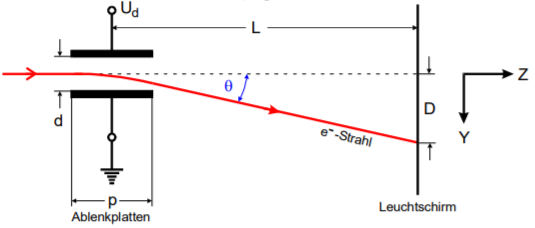
\includegraphics[width=\textwidth]{images/bild2.png}
    \caption{Ablenkung des Elektronenstrahls im Ablenksystem.}
    \label{fig:ablenkung}
\end{figure}

Zwischen den Ablenkplatten herrscht näherungsweise in homogenes Feld, durch dieses werden die Elektronen abgelenkt.
Und daraus folgt der logische Zusammenhang, dass schnellere Teilchen, weniger abgelenkt werden, da sie weniger Zeit im Feld verbringen.
Nach dem Austreten aus dem Feld besitzt ein Elektron die Geschwindigkeit

\begin{equation}
    v_\text{y} = \frac{e_0 \cdot U_\text{d}}{m_0 \cdot d} \cdot \Delta t
    \label{eq:yges}
\end{equation}

in Y Richtung.
Der Ablenkwinkel $\theta$ kann dann über den geometrischen Zusammenhang

\begin{equation}
    \theta = \frac{v_\text{y}}{v_\text{z}}
    \label{eq:theta1}
\end{equation}

oder über 

\begin{equation}
    D = \frac{p L U_\text{d}}{2 d U_\text{B}}
    \label{eq:verschiebung}
\end{equation}

bestimmt werden.

\subsection{Prinzip des Kathodenstrahl-Oszillographen}
\label{ssec:t3}

Durch einige Änderungen kann die Kathodenstrahlröhre zu einem Kathodenstrahl-Oszillographen umfunktioniert werden.
Dafür wird der Teil des Ablenksystems, der in die X-Richtung ablenkt an deine Sägezahnspannung geschaltet und die andere Platte mit der zu messenden Wechselspannung verbunden.
Die beiden Spannungen müssen im Verhältnis 

\begin{equation}
n \cdot \nu _\text{Sä} = m \cdot \nu _\text{We}
    \label{eq:verh}
\end{equation}

stehen, damit auf dem Leuchtschirm der zeitliche Verlauf der Wechselspannung zu sehen ist.
Dabei müssen $n$ und $m$ ganze Zahlen sein.